
%(BEGIN_QUESTION)
% Copyright 2006, Tony R. Kuphaldt, released under the Creative Commons Attribution License (v 1.0)
% This means you may do almost anything with this work of mine, so long as you give me proper credit

In the study of physics we find sets of variables related to one another by differentiation and integration {\it with respect to time}.  Position, velocity, and acceleration are one such set.  Voltage and current in reactive circuits is another set.  Such examples are often given to illustrate differentiation and integration, because most people find it easier to grasp these complex operations in a familiar context.  However, exploring these common relationships makes it easy for new students of calculus to think that differentiation and integration must always have something to do with time, when they in fact this is not necessarily true.

\vskip 10pt

Here is a non-time-related application of integration that is relatively easy to understand and apply: the physics concept of {\it work}.  ``Work'' is the gainful expenditure of energy, calculated in physical terms by the magnitude of applied force multiplied by the displacement (travel) in the direction of that force ($W = F x$).  For example, lifting a 250 pound weight 4 feet off the ground constitutes 1000 foot-pounds of work:

$$\includegraphics[width=15.5cm]{i01574x01.eps}$$

\filbreak

If we graph force and distance to obtain a geometric understanding of work, we see that the multiplication of force and distance may be interpreted as the {\it area} bounded by the graph:

$$\includegraphics[width=15.5cm]{i01574x02.eps}$$

Lifting this weight higher does not change the force required, but it does change the distance, leading to a new calculation of work (a greater area bounded on the graph).

\vskip 10pt

Express work ($W$) as a calculus equation, in terms of the variables force ($F$) and displacement ($x$).  Specifically, express the work calculation for this particular weight-lifting problem.

\vskip 20pt \vbox{\hrule \hbox{\strut \vrule{} {\bf Suggestions for Socratic discussion} \vrule} \hrule}

\begin{itemize}
\item{} Is the hoist in this problem functioning as an energy {\it source} or an energy {\it load}?  How can you tell based on directions of force and displacement vectors? 
\item{} How could you use calculus notation to express the energy {\it released} as the weight is lowered from a height of 4 feet back down to ground level?  Calculate this energy quantity.
\item{} How could you use calculus notation to express the energy required to hoise the weight from a height of 2 feet up to a height of 4 feet?  Calculate this energy quantity.
\item{} Identify the mathematical sign (positive or negative) of force ($F$), differentials of distance ($dx$), and work ($W$) while the weight is being {\it lifted} by the hoist.
\item{} Identify the mathematical sign (positive or negative) of force ($F$), differentials of distance ($dx$), and work ($W$) while the weight is being {\it lowered} by the hoist.
\item{} Modern electric elevators use motors powered via VFDs (Variable Frequency Drives) to precise control the starting, stopping, and speed of the motor for smooth elevator positioning.  Large VFDs provide a very useful feature called {\it regenerative braking} which makes the motor act as a generator when the elevator descends.  Explain why regenerative braking is a useful feature for elevator control.  Is it possible to build an electrically-powered elevator without this feature?
\item{} Compare the amount of energy required to hoist this load 4 feet upwards in 10 seconds, versus the amount of energy required to hoist the load the same distance (4 feet) in half the time (5 seconds).  Explain your analysis of the two energy quantities.
\item{} Define {\it power} as it applies to this scenario, and identify the appropriate calculus function (i.e. either differentiation or integration) for calculating power given the variables available to us.
\end{itemize}

\underbar{file i01574}
%(END_QUESTION)





%(BEGIN_ANSWER)

$$W = \int F \> dx$$

$$1000 \hbox{ ft-lb} = \int_{0\hbox{ ft}}^{4\hbox{ ft}} 250 \hbox{ lb} \> dx$$

%(END_ANSWER)





%(BEGIN_NOTES)



%INDEX% Mathematics, calculus: integral (work)

%(END_NOTES)


